%%%%%%%%%%%%%%%%%%%%%%%%%%%%%%%%%%%%%%%%%
% Classic Lined Title Page 
% LaTeX Template
% Version 1.0 (27/12/12)
%
% This template has been downloaded from:
% http://www.LaTeXTemplates.com
%
% Original author:
% Peter Wilson (herries.press@earthlink.net)
%
% License:
% CC BY-NC-SA 3.0 (http://creativecommons.org/licenses/by-nc-sa/3.0/)
% 
% Instructions for using this template:
% This title page compiles as is. If you wish to include this title page in 
% another document, you will need to copy everything before 
% \begin{document} into the preamble of your document. The title page is
% then included using \titleAT within your document.
%
%%%%%%%%%%%%%%%%%%%%%%%%%%%%%%%%%%%%%%%%%

%----------------------------------------------------------------------------------------
%	PACKAGES AND OTHER DOCUMENT CONFIGURATIONS
%----------------------------------------------------------------------------------------



\documentclass[a4paper]{article}

\usepackage[utf8]{inputenc}
\usepackage{hyperref}
\usepackage{titlesec}
\usepackage{amssymb,amsmath}
\usepackage[italian]{babel}
\usepackage[titles]{tocloft}
\usepackage{appendix}
\hypersetup{%
    pdfborder = {0 0 0}
}
\usepackage{graphicx}
\usepackage[svgnames]{xcolor} % Required to specify font color
\usepackage{eurosym}

\newcommand*{\plogo}{\fbox{$\mathcal{PL}$}} % Generic publisher logo
\usepackage{listings}
\usepackage{fancyhdr}
\usepackage{lastpage}
\usepackage{ragged2e}
\usepackage{listingsutf8}
\usepackage{mathtools}

%----------------------------------------------------------------------------------------
%	TITLE PAGE
%----------------------------------------------------------------------------------------

\newcommand*{\titleAT}{\begingroup % Create the command for including the title page in the document
\newlength{\drop} % Command for generating a specific amount of whitespace
\drop=0.1\textheight % Define the command as 10% of the total text height

\rule{\textwidth}{1pt}\par % Thick horizontal line
\vspace{2pt}\vspace{-\baselineskip} % Whitespace between lines
\rule{\textwidth}{0.4pt}\par % Thin horizontal line

\vspace{\drop} % Whitespace between the top lines and title
\begin{center} % Center all text
\textcolor{Black}{ % Red font color
{\Huge Algoritmi}\\[0.5\baselineskip] % Title line 1
{\Large e}\\[0.75\baselineskip] % Title line 2
{\Huge Strutture Dati}} % Title line 3
\\[2\baselineskip]
{\Large \version{}}

\vspace{0.25\drop} % Whitespace between the title and short horizontal line
\rule{1\textwidth}{0.4pt}\par % Short horizontal line under the title
\vspace{\drop} % Whitespace between the thin horizontal line and the author name

\end{center}
\vfill % Whitespace between the author name and publisher text
\vfill
{\large Luca De Franceschi}
\hfill
{\large Università degli studi di Padova}



%\rule{\textwidth}{0.4pt}\par % Thin horizontal line
%\vspace{2pt}\vspace{-\baselineskip} % Whitespace between lines
%\rule{\textwidth}{1pt}\par % Thick horizontal line

\endgroup}

\titleformat{\chapter}[display]
{}{\hfill\rule{.7\textwidth}{3pt}}{2pt}
{\hspace*{.3\textwidth}\huge\bfseries}[\addvspace{1pt}]
\titleformat{name=\chapter,numberless}[display]
{}{\hfill\rule{.7\textwidth}{3pt}}{2pt}
{\hspace*{.3\textwidth}\huge\bfseries}[\addvspace{1pt}]

\renewcommand*\contentsname{Indice}

\newcommand{\glossario}[1]{\textit{#1\ped{G}}}

\lstset{frame=shadowbox,
  language=c++,
  aboveskip=10mm,
  belowskip=10mm,
  showstringspaces=false,
  columns=flexible,
  basicstyle={\small\ttfamily},
  numbers=none,
  numberstyle=\tiny\color{gray},
  keywordstyle=\color{blue},
  commentstyle=\color{gray},
  stringstyle=\color{red},
  breaklines=true,
  breakatwhitespace=true
  tabsize=1
}
\lstset{inputencoding=utf8/latin1}

\renewcommand{\lstlistingname}{Listato}
\renewcommand{\footrulewidth}{0.4pt}

\newcommand{\changefont}{%
    \fontsize{5}{7}\selectfont
}

\def\arraystretch{2}

\DeclarePairedDelimiter\ceil{\lceil}{\rceil}
\DeclarePairedDelimiter\floor{\lfloor}{\rfloor}

%----------------------------------------------------------------------------------------
%	CONSTANTS
%----------------------------------------------------------------------------------------

\newcommand{\version}{v0.8.0}

\newcommand{\authorName}{Luca De Franceschi}

%----------------------------------------------------------------------------------------
%	DOCUMENT HEADER
%----------------------------------------------------------------------------------------

\begin{document}
\titleAT % This command includes the title page
\pagestyle{empty}
\newpage
\section*{Diario delle modifiche}

\begin{center}

	\begin{table}[htpd]
		\begin{tabular}{| l | l | l | p{50mm} |}
			\hline
			\hline
			\textbf{Autore} & \textbf{Versione} & \textbf{Data} & \textbf{Descrizione} \\
			\hline
			\hline
			Luca De Franceschi & 0.8.0 & 16/06/2014 & Inserito capitolo codici di Huffman \\ \hline
			Luca De Franceschi & 0.7.0 & 15/06/2014 & Inserito capitolo hashing e risposte a domande degli appelli \\ \hline
			Luca De Franceschi & 0.6.0 & 14/06/2014 & Inserito capitolo algoritmi golosi con esercizio del pulmino \\ \hline
			Luca De Franceschi & 0.5.0 & 13/06/2014 & Inserito capitolo analisi ammortizzata con due esercizi, incrementata sezione metodo dell'integrale \\ \hline
			Luca De Franceschi & 0.4.0 & 11/06/2014 & Inserito capitolo analisi complessità con metodo dell'integrale e metodo dell'esperto \\ \hline
			Luca De Franceschi & 0.3.0 & 11/06/2014 & Inserita spiegazione metodo di sostituzione \\ \hline
			Luca De Franceschi & 0.2.0 & 11/06/2014 & Inserita teoria su programmazione dinamica \\ \hline
			Luca De Franceschi & 0.1.0 & 11/06/2014 & Creata struttura del documento \\ \hline
		\end{tabular}
	\end{table}
	
\end{center}
\tableofcontents
\clearpage

%----------------------------------------------------------------------------------------
%	HEADER FORMAT
%----------------------------------------------------------------------------------------

\fancyhf{}
\fancyhead[RE]{\small\scshape\nouppercase{\leftmark}}
\fancyhead[LO]{\small\scshape\nouppercase{\rightmark}}
\fancyhead[LE,RO]{\small\thepage}
\lhead{\rightmark}
\rhead{Algoritmi e strutture dati}
\rfoot{\thepage/\pageref{LastPage}}
\lfoot{\authorName}

\pagestyle{fancy}


%----------------------------------------------------------------------------------------
%	CONTENT
%----------------------------------------------------------------------------------------

\raggedright

\section{Stima della complessità di un algoritmo}

Identifichiamo dei casi base, studiando la complessità degli algoritmi noti.

\begin{enumerate}

\item Le operazioni elementari, messe al di fuori dei cicli, e che riguardano l'uso di variabili hanno complessità costante $c_i$, aprossimabile a 0 nello studio della complessità asintotica;

\item Da \textit{insertion-sort} si vede che un \textit{for i = 2 to n} ha complessità pari a $n$. Constatiamo dunque che un ciclo for che va dall'indice $1$ all'indice $n$ avrà complessità $c_i(n+1)$;

\item Tutte le operazioni elementari che compaiono all'interno di un ciclo for di complessità $c_i(n+1)$ hanno complessità $c_in$;

\item Per i cicli annidati in altri cicli a complessità è data da $c_i\sum_{j=x}^{n}(c_j)$, dove gli estremi della sommatoria sono gli estremi del del ciclo esterno.

\end{enumerate}

Per valutare la complessità si scrive l'equazione $T(n)$ sommando tutte le complessità. Per studiare le sommatorie si utilizza il \textbf{metodo dell'integrale}.

\subsection{Metodo dell'integrale}

Se $f(x)$ è una funzione \textbf{non decrescente}:

$$\int_a^{b+1} f(x)\mathrm{d}x\le \sum_{i=a}^b f(i) \le \int_{a-1}^{b+1} f(x)\mathrm{d}x$$

Se $f(x)$ è una funzione \textbf{non decrescente}:

$$\int_a^{b+1} f(x)\mathrm{d}x \le \sum_{i=a}^b f(i) \le \int_{a-1}^b f(x)\mathrm{d}x$$

Inoltre riportiamo di seguito le comuni sommatorie:

\begin{itemize}

\item \textbf{Serie aritmetica}: $\sum_{i=1}^n i = \frac{n(n+1)}{2}$;
\item \textbf{Serie geometrica}: $\sum_{i=0}^k q^i = \frac{q^{k+1}-1}{q-1}$ \hfill $q\neq1$

\end{itemize}

\subsection{Andamento asintotico}

Una volta ottenuta una funzione che rappresenta la complessità dell'algoritmo ci può interessare prendere in esame l'andamento asintotico della medesima. Per farlo introduciamo le seguenti notazioni:

\begin{itemize}

\item \textbf{``$O$'' grande}: date due funzioni $f(n)$ e $g(n)$ si dice che $f(n)$ è ``$O$'' grande di $g(n)$ se esiste un $c>0$ e un $h_0$ tali che: 

$$f(n)\le cg(n)$$ 

per $n\ge h_0$ (\textbf{limite asintotico superiore}). In pratica l'ordine di crescita di $f(n)$ è non superiore a quello di $g(n)$;

\item \textbf{``$\Omega$'' grande}: date $f(n)$ e $g(n)$ si dice che $f(n)$ è ``$\Omega$'' grande di $g(n)$ se esiste una costante $c>0$ e un $h_0$ tale che:

$$f(n)\ge cg(n)$$ 

per $n\ge h_0$ (\textbf{limite asintotico inferiore}). In pratica l'ordine di crescita di $f(n)$ è non inferiore a quello di $g(n)$;

\item \textbf{``$\Theta$'' grande}: date $f(n)$ e $g(n)$ si dice che $f(n)$ è ``$\Theta$'' grande di $g(n)$ se ci sono costanti positive $c_1$, $c_2$ e un $h_0$ tali che:

$$c_1g(n)\le f(n) \le c_2g(n)$$

per $n\ge h_0$ (\textbf{limite asintotico stretto}). In pratica diciamo che se $f(n)=O(g(n))$ e $f(n)=\Omega(g(n))$ allora è vero anche che $f(n)=\Theta(g(n))$

\end{itemize}

Di una funzione non ci interessa la sua forma ma il suo comportamento asintotico. Spesso è possibile determinare dei limiti asintotici calcolando il limite di un rapporto:

$$\lim_{n \to \infty} \frac{f(n)}{g(n)}$$

In base al risultato di questo limite ho tre casi:

\begin{enumerate}

\item Ottengo un valore costante $k>0$: in questo caso $f(n)$ è dello stesso ordine di $g(n)$, e dunque:

$$\forall \epsilon>0, \exists h_0 | h\ge h_0 : k-\epsilon \le f(n)/g(n)\le k+\epsilon$$

ponendo:

$$c_1g(n)\le f(n) \le c_2g(n)$$

Dunque concludo dicendo che $f(n)=\Theta(g(n))$;

\item Il limite tende a $\infty$: $f(n)=\Omega(g(n))$;
\item Il limite tende a $0$: $f(n)=O(g(n))$.

\end{enumerate}

\subsection{Metodo dell'esperto}

Per risolvere le ricorrenze il primo metodo da utilizzare è il \textbf{metodo dell'esperto}. Se la ricorrenza è espressa nella forma:

$$T(n)=aT(n/b)+f(n)$$

e se $a \ge 1$ e $b<1$ allora:

\begin{enumerate}

\item Tolgo eventuali arrotondamenti;
\item Calcolo $\log_ba$ e calcolo il limite: $\lim_{n \to \infty}\frac{f(n)}{n^{\log_ba}}$;

\end{enumerate}

A questo punto, in base al valore del limite ho 3 possibili casi:

\subsubsection{Caso 2}

Se il limite è \textbf{finito} e diverso da zero:

$$f(n)=\Theta(n^{\log_ba})\Rightarrow T(n)=\Theta(n^{\log_ba}\log n)$$

\subsubsection{Caso 1}

Se il limite è \textbf{uguale a zero} devo trovare un valore $\epsilon > 0$ per il quale risulta finito il limite:

$$\lim_{n \to \infty}\frac{f(n)}{n^{\log_ba-\epsilon}}=k$$

Se lo trovo allora posso affermare che:

$$f(n)=O(n^{\log_ba-\epsilon}) \Rightarrow T(n)=\Theta(n^{\log_ba})$$

\subsubsection{Caso 3}

Se il limite è $\int$ allora devo trovare un $\epsilon >0$ per il quale risulti:

$$\lim_{n \to \infty}\frac{f(n)}{n^{\log_ba+\epsilon}}\neq 0$$

Se lo trovo allora devo studiare l'equazione:

$$af(n/b)\le k(f(n))$$

se trovo un $k<1$ allora posso concludere che:

$$f(n)=\Omega(n^{\log_ba+\epsilon})\Rightarrow T(n)=\Theta(f(n))$$

\subsection{Metodo di sostituzione}

Se non riesco ad applicare il metodo dell'esperto allora devo utilizzare il \textbf{metodo di sostituzione}.

Per capire il metodo di sostituzione proviamo a risolvere il seguente esercizio:
\linebreak
\linebreak
La ricorrenza $T(n)=4T(n/2)+n^2\log n$ si può risolvere con il metodo dell'esperto? Giustificare la risposta. Se la risposta è negativa usare il metodo di sostituzione per dimostrare che $T(n)=O(n^2\log^2n)$.
\linebreak
\linebreak
Anzitutto vediamo i dati a disposizione:

$$a = 4, b = 2$$ 
$$f(n)=n^2\log n$$
$$g(n)=n^{\log_{b}a}=n^{\log_{2}4}=n^2$$

Calcoliamo ora il limite:

$$\lim_{n \to +\infty}\frac{n^2\log n}{n^2}=\infty$$

Da cui deduco che:

$$f(n)=\Omega(n^2)$$

Potrei dunque essere nel caso 3. Devo trovare un $$\epsilon > 0$$  tale che:

$$\lim_{n \to +\infty}\frac{n^2\log n}{n^{2+\epsilon}}\neq0$$

Ma mi accorgo subito che la cosa è impossibile, in quanto il denominatore, incrementando l'esponente, crescerà molto più velocemente rispetto al numeratore, per cui avrò sempre un valore tendente allo zero. Da questa considerazione deduco che la ricorrenza \textbf{non è risolvibile con il metodo dell'esperto}.
\linebreak
\linebreak
Procedo dunque con la sostituzione. Proviamo $T(n)=O(n^2\log^2n)$. Assumiamo che per un'opportuna costante $C>1$ e $\forall x<n$ sia verificata la disuguaglianza $T(x)\le C(x^2\log^2x)$ e dimostriamo che vale anche per $n$:

$$T(n)=4T(n/2)+n^2\log n \le 4C(n/2)^2\log^2(n/2)+n^2\log n$$
$$=Cn^2(\log n -1)^2+n^2\log n$$
$$=Cn^2(\log^2n-2\log n+1)+n^2\log n$$
$$=Cn^2\log^2n-2Cn^2\log n +Cn^2\log n+Cn^2+n^2\log n$$
$$=Cn^2\log^2n-(C-1)n^2\log n-Cn^2(\log n -1)$$

Ora applico una \textbf{maggiorazione}:

$$\le Cn^2\log^2n$$

Dunque ho dimostrato che: $T(n)=O(n^2\log^2n)$
\section{Hashing}

Molte operazioni richiedono un insieme dinamico che supporta soltanto le operazioni di dizionario \textit{INSERT}, \textit{SEARCH} e \textit{DELETE}. Una \textbf{tavola hash} è una struttura dati efficace per implementare i \textbf{dizionari}. Sebbene la ricerca di un elemento in una tavola hash richieda, nel caso peggiore, lo stesso tempo $\Theta(n)$ richiesto per cercare un elemento in una lista concatenata, l'hashing si comporta molto bene nella pratica. Sotto ipotesi ragionevoli, il tempo medio per cercare un elemento in una tavola hash è $O(1)$.
Una tavola hash è una generalizzazione della nozione più semplice di array ordinario. Quando il numero di \textbf{chiavi} effettivamente memorizzate è piccolo rispetto al numero totale di chiavi possibili, le tavole hash diventano una valida alternativa all'indirizzamento diretto di un array, in quanto una tavola hash tipicamente usa un array di dimensione proporzionale al numero di chiavi effettivamente memorizzate.

\subsection{Tavole a indirizzamento diretto}

L'indirizzamento diretto è una tecnica semplice che funziona bene quando l'universo $U$ delle chiavi è ragionevolmente \textbf{piccolo}. 
Per rappresentare l'insieme dinamico, utilizziamo un array o \textbf{tavola a indirizzamento diretto}, che indicheremo con $T[0...m-1]$, dove ogni posizione o \textbf{cella} corrisponde a una chiave nell'universo $U$. La cella $k$ punta ad un elemento dell'insieme con chiave $k$. Se l'insieme non contiene l'elemento con chiave $k$, allora $T[k]=nil$.

\begin{figure}[htpd]
\centering
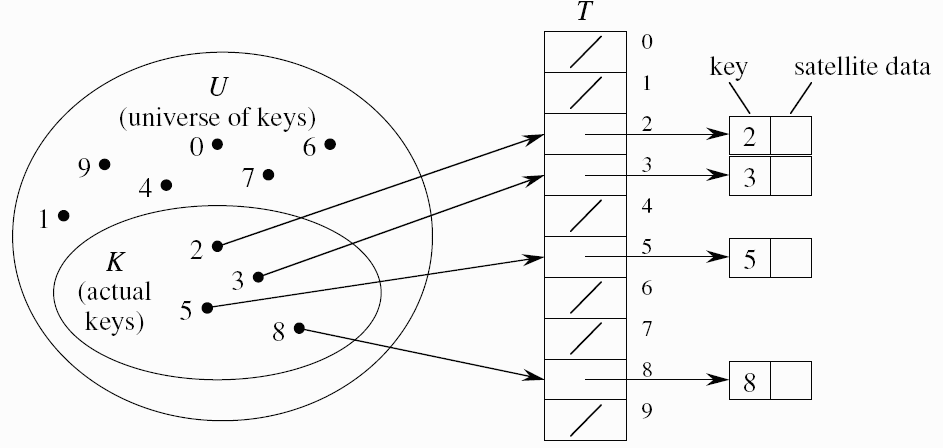
\includegraphics[width=100mm]{images/direct-hash.png}
\caption{Tavola a indirizzamento diretto}
\end{figure}

\begin{lstlisting}

DIRECT-ADDRESS-SEARCH (T, k)
	return T[k]

\end{lstlisting}

\begin{lstlisting}

DIRECT-ADDRESS-INSERT (T,x)
	T[x.key] = x

\end{lstlisting}

\begin{lstlisting}

DIRECT-ADDRESS-DELETE (T, x)
	T[x.key] = nil

\end{lstlisting}

Ciascuna di queste operazioni richiede tempo $O(1)$.

\subsection{Tavole hash}

La difficoltà dell'indirizzamento diretto è ovvia: se l'universo $U$ delle chiavi è troppo grande, memorizzare una tavola $T$ di dimensione $|U|$ può essere impraticabile. Inoltre, l'insieme $K$ delle chiavi \textit{effettivamente memorizzate} può essere così piccolo rispetto a $U$ che la maggior parte dello spazio allocato per la tavola $T$ sarebbe sprecato.

Con l'indirizzamento diretto un elemento con chiave $k$ è memorizzato nella cella $k$. Con l'hashing, questo elemento è memorizzato nella cella $h(k)$: cioè utilizziamo una \textbf{funzione hash} $h$ per calcolare la cella dalla chiave $k$. Qui $h$ associa l'universo $U$ delle chiavi alle celle di una \textbf{tavola hash} $T[0...m-1]$:

$$h:U\to \{0,1,...,m-1\}$$

dove la dimensione $m$ della tavola hash è generalmente molto più piccola di $|U|$. Diciamo che un elemento con chiave $k$ viene mappato nella cella $h(k)$ o anche che $h(k)$ è il \textbf{valore hash} della chiave $k$.

Il compito della funzione hash è quello di ridurre l'intervallo degli indici e di conseguenza la dimensione dell'array. L'array ha dimensione $m$ invece di $|U|$.

\begin{figure}[htpd]
\centering
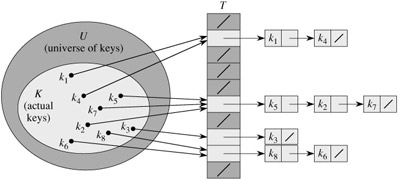
\includegraphics[width=100mm]{images/hashing.jpg}
\caption{Utilizzo di una funzione hash}
\end{figure}

C'è un problema: due chiavi possono essere mappate nella stessa cella. Questo evento si chiama \textbf{collisione}. Fortunatamente ci sono tecniche efficaci per risolvere i conflitti creati dalle collisioni.

\subsubsection{Risoluzione delle collisioni mediante concatenamento}

Nel \textbf{concatenamento} poniamo tutti gli elementi che sono associati alla stessa cella in una lista concatenata. La cella contiene un puntatore alla testa della lista di tutti gli elementi memorizzati che vengono mappati in $j$; se non ce ne sono, la cella $j$ contiene la costante $nil$. Le operazioni di dizionario sono facili da implementare:

\begin{lstlisting}

CHAINED-HASH-INSERT (T, x)
	inserisce x in testa alla lista T[h(x.key)]

\end{lstlisting}

\begin{lstlisting}

CHAINED-HASH-SEARCH (T, x)
	ricerca un elemento con chiave k nella lista T[h(k)]

\end{lstlisting}

\begin{lstlisting}

CHAINED-HASH-DELETE (T, x)
	cancella x dalla lista T[h(x.key)]

\end{lstlisting}

Il tempo di esecuzione nel caso peggiore per l'inserimento è $O(1)$.

\subsubsection{Analisi dell'hashing con concatenamento}

Data una tavola hash $T$ con $m$ celle dove sono memorizzati $n$ elementi, definiamo \textbf{fattore di carico} $\alpha$ della tavola $T$ il rapporto $n/m$, ossia il numero medio di elementi memorizzati in una lista.

Il comportamento nel caso peggiore dell'hashing con concatenamento è pessimo: tutte le $n$ chiavi sono associate alla stessa cella, creando una lista di lunghezza $n$. Il tempo di esecuzione della ricerca è quindi $\Theta(n)$, più il tempo per calcolare la funzione hash.

Le prestazioni dell'hashing nel caso medio dipendono dal modo in cui la funzione hash $h$ distribuisce mediamente l'insieme delle chiavi da memorizzare tra le $m$ celle. Per adesso supponiamo che qualsiasi elemento abbia la stessa probabilità di essere mandato in una qualsiasi delle $m$ celle, indipendentemente dalle celle in cui sono mandati gli altri elementi. Questa ipotesi è detta \textbf{hashing uniforme semplice}.

\subsubsection*{Teorema}

In una tavola hash le cui collisioni sono risolte con il concatenamento, una ricerca senza successo richiede un tempo $\Theta(1+\alpha)$ nel caso medio, nell'ipotesi di hashing uniforme semplice.

\subsubsection*{Teorema}

In una tavola hash le cui collisioni sono risolte con il concatenamento, una ricerca con successo richiede un tempo $\Theta(1+\alpha)$ nel caso medio, nell'ipotesi di hashing uniforme semplice
\linebreak
\linebreak
Se il numero di celle della tavola hash è almeno proporzionale al numero di elementi della tavola, abbiamo $n = O(m)$ e, di conseguenza, $\alpha=n/m=O(m)/m=O(1)$ nel caso peggiore e la cancellazione richiede il tempo $O(1)$ nel caso peggiore quando le liste sono doppiamente concatenate, tutte le operazioni di dizionario possono essere svolte, in media, nel tempo $O(1)$.

\subsection{Funzioni hash}

Una buona funzione hash soddisfa l'ipotesi dell'hashing uniforme semplice: ogni chiave ha la stessa probabilità di essere mandata in una qualsiasi delle $m$ celle, indipendentemente dalla cella cui viene mandata qualsiasi altra chiave.

Purtroppo, di solito non è possibile verificare questa condizione, in quanto raramente è nota la distribuzione delle probabilità secondo la quale vengono estratte le chiavi. Ad esempio se le chiavi sono numeri reali casuali $k$ distribuiti in modo indipendente e uniforme nell'intervallo $0\le k < 1$, la funzione hash:

$$h(k)=\floor*{km}$$

soddisfa la condizione dell'hashing uniforme semplice.

La maggior parte delle funzioni hash suppone che l'universo delle chiavi sia l'insieme dei numeri naturali: $\mathbb{N}=\{0,1,2,...\}$. Quindi se le chiavi non sono numeri naturali, occorre un metodo per interpretarle come tali.

\subsubsection{Il metodo della divisione}

Quando si applica il \textbf{metodo della divisione} per creare una funzione hash, una chiave $k$ viene associata ad una delle $m$ celle prendendo il resto della divisione fra $k$ ed $m$, cioè la funzione hash è:

$$h(k)=k\mod m$$

Un numero primo non troppo vicino a una potenza esatta di 2 è spesso una buona scelta per $m$. Per esempio supponiamo di allocare una tavola hash per contenere circa $n=2000$ stringhe di caratteri, dove ogni carattere ha 8 bit. Poichè riteniamo accettabile esaminare in media 3 elementi in una ricerca senza successo, allochiamo una tavola hash di dimensione $m=701$. Abbiamo scelto 701 perchè è un numero primo vicino a 2000/3, ma non a una potenza di 2. Trattando ogni chiave $k$ come un numero intero, la funzione hash diventa:

$$h(k)=k\mod 701$$

\subsubsection{Il metodo della moltiplicazione}

Il \textbf{metodo della moltiplicazione} per creare funzioni hash si svolge in due passi. Prima moltiplichiamo la chiave $k$ per una costante $A$ nell'intervallo $0<A<1$ ed estraiamo la parte frazionaria di $kA$. Poi moltiplichiamo questo valore per $m$ e prendiamo la parte intera inferiore del risultato. In sintesi la funzione hash è:

$$h(k)=\floor*{m(kA\mod 1)}$$

Un vantaggio del metodo di moltiplicazione è che non è critico. Tipicamente, lo scegliamo come una potenza di 2 ($m=2^p$ per qualche intero $p$), il che rende semplice implementare la funzione hash nella maggior parte dei calcolatori.

\subsection{Indirizzamento aperto}

Nell'\textbf{indirizzamento aperto}, tutti gli elementi sono memorizzati nella tavola hash stessa; ovvero ogni cella della tavola contiene un elemento dell'insieme dinamico o la costante $nil$. Quando cerchiamo un elemento, esaminiamo sistematicamente le celle della tavola finchè non troviamo l'elemento desiderato o finchè non ci accorgiamo che l'elemento non si trova nella tavola.s

Diversamente dal concatenamento non ci sono nè liste nè elementi memorizzati all'esterno della tavola, quindi la tavola può ``riempirsi'' al punto tale che non possono essere effettuati altri inserimenti. Una conseguenza è che il fattore di carico $\alpha$ non supera mai 1.

Il vantaggio dell'indirizzamento aperto sta nel fatto che esclude completamente i puntatori. Anzichè seguire i puntatori, \textit{calcoliamo} la sequenza delle celle da esaminare. La memoria extra liberata per non aver memorizzato i puntatori offre alla tavola hash un maggior numero di celle, a parità di memoria occupata, consentendo potenzialmente di ridurre il numero di collisioni e di accelerare le operazioni di ricerca.

Per effettuare un inserimento mediante l'indirizzamento aperto, esaminiamo in successione le posizioni della tavola hash (\textbf{ispezione}), finchè non troviamo una cella vuota in cui inserire la chiave. La sequenza delle posizioni esaminate durante un'ispezione \textit{dipende dalla chiave da inserire}.

Con l'indirizzamento aperto si richiede che, per ogni chiave $k$, la \textbf{sequenza di ispezione}:

$$\langle h(k,0),h(k,1),...,h(k,m-1)\rangle$$

sia una permutazione di $\langle 0,1,...,m-1\rangle$, in modo che ogni posizione della tavola hash possa essere considerata come possibile cella in cui inserire una nuova chiave mentre la chiave si riempe.

\subsubsection{Ispezione lineare}

Data una funzione hash ordinaria $h':U\to \{0,1,...,m-1\}$, che chiameremo \textbf{funzione hash ausiliaria}, il metodo dell'\textbf{ispezione lineare} usa la funzione hash:

$$h(k,i)=(h'(k)+i)\mod m$$

per $i=0,1,...,m-1$.

L'ispezione lineare è facile da implementare, ma presenta un problema noto come \textbf{addensamento primario}: si formano lunghe file di celle occupate, che aumentano il tempo medio di ricerca.

\subsubsection{Ispezione quadratica}

L'\textbf{ispezione quadratica} usa una funzione hash della forma:

$$h(k,i)=(h'(k)+c_1i+c_2i^2)\mod m$$

dove $h'$ è una funzione hash ausiliaria, $c_1$ e $c_2\neq 0$ sono costanti ausiliarie e $i=0,1,...,m-1$. La posizione iniziale esaminata è $T[h'(k)]$; le posizioni successivamente esaminate sono distanziate da quantità che dipendono in modo quadratico dal numero di ispezione $i$. Questa tecnica funziona molto meglio dell'ispezione lineare, ma per fare pieno uso della tavola hash, i valori di $c_1$, $c_2$ ed $m$ non si possono scegliere arbitrariamente.

\subsubsection{Doppio hashing}

Il doppio hashing è uno dei metodo migliori disponibili per l'indirizzamento aperto, perchè le permutazioni prodotte hanno molte delle caratteristiche delle permutazioni scelte a caso. Il \textbf{doppio hashing} usa una funzione hash della forma:

$$h(k,i)=(h_1(k)+ih_2(k))\mod m$$

dove $h_1$ e $h_2$ sono funzioni hash ausiliarie. L'ispezione inizia dalla posizione $T[h_1(k)]$; le successive posizioni sono distanziate dalle precedenti posizioni di una quantità $h_2(k)$, modulo $m$. Quindi, diversamente dal caso dell'ispezione linare o quadratica, la sequenza di ispezione qui dipende in due modi dalla chiave $k$, perchè possono variare sia la posizione iniziale di ispezione sia la distanza fra due posizioni successive di ispezione.

Il valore $h_2(k)$ dev'essere relativamente primo con la dimensione $m$ della tavola hash perchè venga ispezionata l'intera tavola hash. Un modo pratico per garantire questa condizione è scegliere $m$ potenza di 2 e definire $h_2$ in modo che produca sempre un numero dispari.

\subsection{Domande}

\subsubsection*{Domanda 1}

Spiegare cos'è l'ipotesi di hash uniforme semplice. Come bisogna scegliere la funzione hash perchè tale ipotesi sia soddisfatta?
\linebreak
\linebreak
\textbf{Risposta}: l'ipotesi di hash uniforme semplice assume che una chiave da inserire nella tavola abbia uguale probabilità di finire in una qualsiasi delle celle della tavola, indipendentemente dalle chiavi inserite precedentemente. Poichè sia soddisfatta tale ipotesi, occorre scegliere la funzione hash tenendo conto della distribuzione di probabilità delle chiavi in input. Alternativamente possiamo scegliere casualmente la funzione hash in un insieme universale.

\subsubsection*{Domanda 2}

Sia $h(k)$ una funzione hash che mappa un insieme $U$ di chiavi in una tavola hash di $m$ celle. Mostrare che esiste una cella in cui la funzione hash manda almeno $\ceil{|U|/m}$ chiavi distinte.
\linebreak
\linebreak
\textbf{Risposta}: se la funzione hash $h(k)$ mandasse al più $\ceil{|U|/m}-1$ chiavi, in ogni cella dovremmo avere al massimo $m(\ceil{|U|/m})$ chiavi. Sia $|U|=qm+r$, con $q$ ed $r$ quoziente e resto della divisione per $m$. Se $r=0$ allora $m(\ceil{|U|/m}-1)=|U|-1<|U|$: assurdo. Se $r>0$ allora $m(\ceil{|U|/m}-1)=mq<|U|$: assurdo. Deve quindi esistere almeno una cella in cui la funzione hash $h(k)$ manda almeno $\ceil{|U|/m}$ chiavi.

\subsubsection*{Domanda 3}

Una tavola hash con risoluzione delle collisioni mediante liste, usa la funzione hash $h(k)=k\mod 257$. Tale tavola hash viene usata per memorizzare delle stringhe di caratteri ASCII. Mostrare che se la stringa $y$ è ottenuta dalla stringa $x$ permutandone i caratteri di posto pari allora $x$ ed $y$ vengono messe nella stessa cella.
\linebreak
\linebreak
\textbf{Risposta}: siccome $256\mod 257 \equiv 1$ e quindi $256^i\mod 257 \equiv (-1)^i$ abbiamo che:

$$h(k)=k\mod 257=(\sum_{i=0}^nc_i(-1)^i)\mod 257=$$
$$=(\sum_{i=0}^nc_i(-1)^i)\mod 257$$

I caratteri di posto pari risultano tutti moltiplicati per 1 e quindi per la commutatività della somma, permutandoli tra loro non cambia il valore di $h(k)$.

\subsubsection*{Domanda 4}

Dire perchè in una tavola hash con indirizzamento aperto non è possibile eliminare un elemento ponendo il valore $nil$ nella cella ma occorre introdurre un nuovo valore $deleted$ diverso sia da $nil$ che da ogni chiave.
\linebreak
\linebreak
\textbf{Risposta}: Se l'elemento eliminato non è l'ultimo elemento della sequenza di ispezione a cui esso appartiene, ponendo il valore a $nil$ nella cella la ricerca degli elementi successivi (che non sono stati rimossi) si ferma non appena trova il valore $nil$ e dà risultato negativo.

\subsubsection*{Domanda 5}

Spiegare il fenomeno dell'addensamento primario in una tavola hash con indirizzamento aperto e che usa l'ispezione lineare.
\linebreak
\linebreak
\textbf{Risposta}: L'ispezione lineare usa la funzione hash:

$$h(k,i)=(h'(k)+1)\mod m$$

assumendo che $h'(k)$ soddisfi l'ipotesi di hash uniforme semplice, se la tavola è vuota l'inserimento della prima chiave può avvenire con uguale probabilità $1/m$ in una qualsiasi delle $m$ celle della tavola. Ma essendo la cella $h'(k_1)$ occupata dalla chiave $k_1$, se $h'(k_2)=h'(k_1)$ la chiave $k_2$ viene rimandata nella cella successiva $h'(k_1)+1$. Di conseguenza la probabilità che $k_2$ venga mandata nella cella $h'(K_1)+1$ è doppia, ossia pari a $2/m$. In generale, se una cella libera è preceduta da $n$ celle consecutive occupate, la probabilità che la prossima chiave venga messa in tale cella è pari ad $(n+1)/m$. Di conseguenza sequenze consecutive di celle occupate tendono ad allungarsi sempre di più.

\subsubsection*{Domanda 6}

Come la domanda 1 ma con $h(k)=k\mod 17$, e con $y$ ottenuta da $x$ permutando i caratteri.
\linebreak
\linebreak
\textbf{Risposta}: siccome $256^i\mod 17 = 1$ abbiamo che:

$$h(k)=k\mod 17 = (\sum_{i=0}^nc_i256^i)\mod 17=(\sum_{i=0}^nc_i)\mod 17$$

Per la commutatività della somma, permutando i caratteri non cambia il valore di $h(k)$.


\section{Programmazione dinamica}

In maniera del tutto generale la programmazione dinamica può essere descritta nel seguente modo:

\begin{enumerate}

\item Identifichiamo dei \textbf{sottoproblemi} del problema originario e utilizziamo una \textit{tabella} per memorizzare i risultati intermedi;
\item Inizialmente vanno definiti i \textbf{valori iniziali} di alcuni elementi della tabella, corrispondenti a sottoproblemi più semplici;
\item Al generico passo, avanziamo in modo opportuno sulla tabella calcolando il valore della soluzione di un sottoproblema in base alla soluzione di sottoproblemi precedentemente risolti (corrispondenti ad elementi della tabella precedentemente calcolati);
\item Alla fine restituiamo la soluzione del problema originario, che è stato memorizzato in un particolare elemento della tabella.

\end{enumerate}

La programmazione dinamica è usata normalmente per \textbf{problemi di ottimizzazione}, il termine ``programmazione'' si riferisce al metodo tabulare, non alla scrittura di codice.
\linebreak
\linebreak
La programmazione è applicabile con vantaggi se:

\begin{itemize}

\item Gode della proprietà di \textbf{sottostruttura ottima}: una soluzione si può costruire a partire da soluzioni ottime di sottoproblemi;
\item Il numero di sottoproblemi distinti è molto minore del numero di soluzioni possibili tra cui cercare quella ottima, altrimenti c'è la \textbf{ripetizione di sottoproblemi}, ovvero se il numero di sottoproblemi distinti è molto minore del numero di soluzioni possibili tra cui cercare quella ottima, allora uno stesso sottoproblema deve comparire molte volte come sottoproblema di altri sottoproblemi.

\end{itemize}

\subsection*{Ordine di calcolo delle soluzioni dei sottoproblemi}

\textbf{Bottom-up}: le soluzioni dei sottoproblemi del problema in esame sono già state calcolate. È il metodo migliore se per il calcolo della soluzione globale servono le soluzioni di tutti i sottoproblemi.
\linebreak
\linebreak
\textbf{Top-down}: è una procedura ricorsiva che dall'alto scende verso il basso. È la soluzione migliore se per il calcolo della soluzione globale servono soltanto alcune delle soluzioni dei sottoproblemi.
\section{Algoritmi golosi}

Si parla sempre di \textbf{problemi di ottimizzazione}.

\begin{figure}[htbp]
\centering
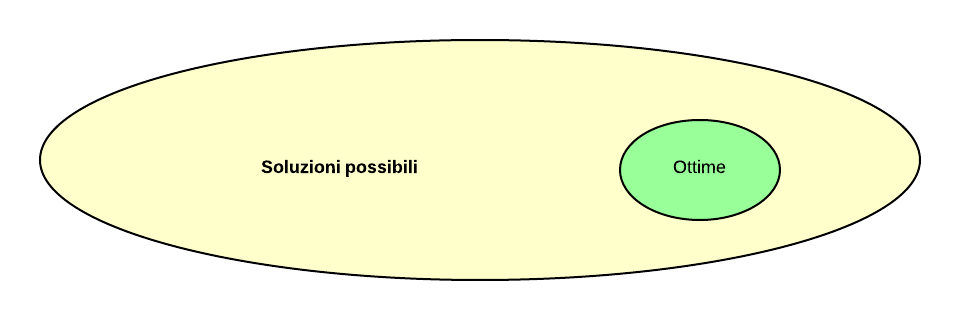
\includegraphics[width=100mm]{images/gready1.png}
\caption{Soluzioni di un problema}
\end{figure}

Se utilizziamo l'\textbf{enumerazione esaustiva}:

\begin{itemize}

\item Si generano tutte le soluzioni possibili;
\item Si calcola il costo di ciascuna di esse;
\item Se ne seleziona una di ottima.

\end{itemize}

Questo metodo è chiaramente efficace ma comporta \textbf{tempi esponenziali}, perchè l'insieme delle soluzioni è generalmente enorme.
\linebreak[2]
Un \textbf{algoritmo goloso} sceglie sempre una soluzione \textbf{localmente ottima}:

\begin{figure}[htpd]
\centering
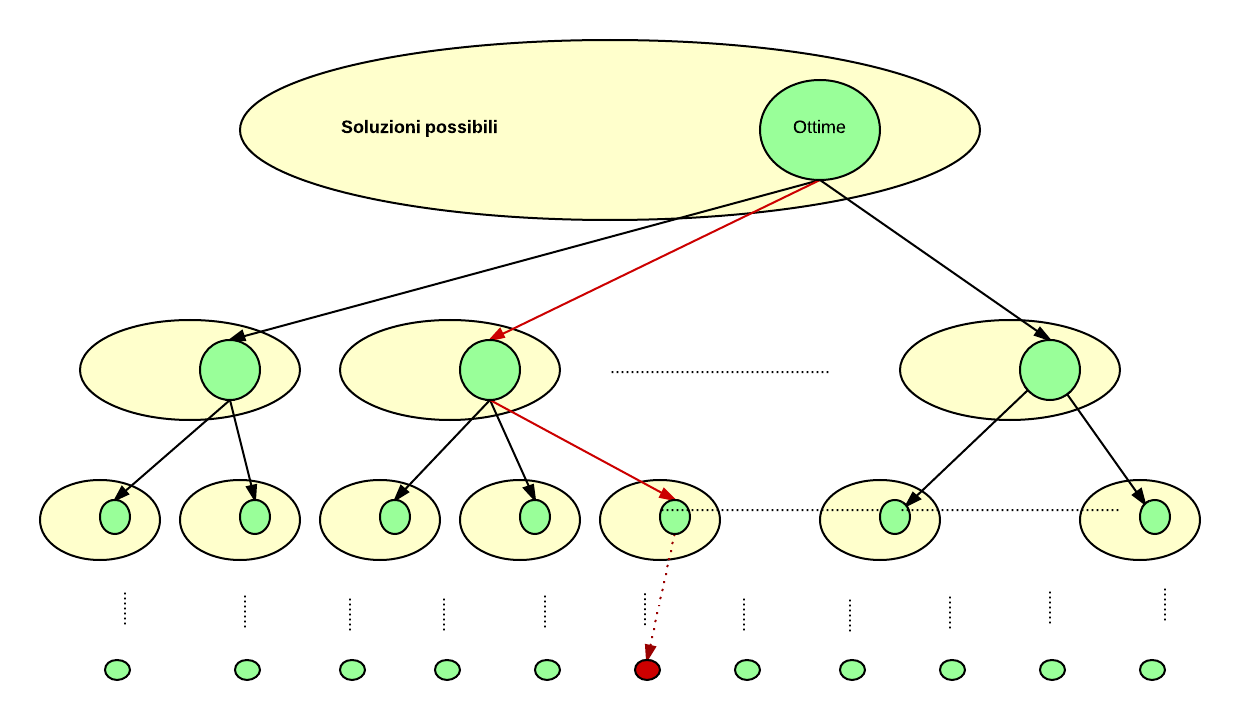
\includegraphics[width=130mm]{images/gready2.png}
\caption{Schema di un algoritmo goloso}
\end{figure}

\begin{enumerate}

\item Ogni volta si fa una scelta che sembra migliore localmente;
\item In questo modo per alcuni problemi si ottiene una soluzione globalmente ottima.

\end{enumerate}

\subsection{Problema della scelta di attività}

Un esempio tipico è quello del \textbf{problema della scelta di attività}. Supponiamo di avere a disposizione $n$ attività $a_1,a_2,...,a_n$ che utilizzano la stessa risorsa (ad esempio un'aula). Ciascuna attività ha un tempo di inizio $s_i$ e un tempo di fine $f_i$, con $0\le s_i < f_i < \infty$.

$a_i$ occupa la risorsa nell'intervallo $[s_i,f_i)$.

$a_i$ e $a_j$ sono \textbf{compatibili} se gli intervalli $[s_i,f_i)$ e $(s_j,f_j]$ sono disgiunti.
\linebreak[2]
Strategie golose:

\begin{itemize}

\item Scegliere l'attivitò che inizia per prima:

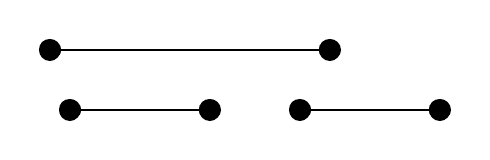
\includegraphics[width=50mm]{images/activity1.png}

Non funziona!

\item Scegliere l'attività che dura meno tempo:

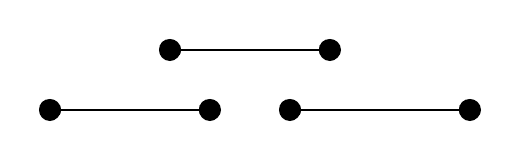
\includegraphics[width=50mm]{images/activity2.png}

Non funziona!

\item Scegliere l'attività incompatibile con il minor numero di altre attività:

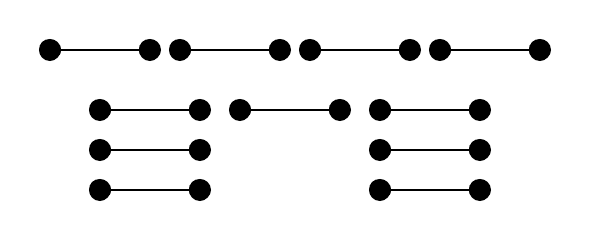
\includegraphics[width=50mm]{images/activity3.png}

Non funziona!

\end{itemize}

La strategia che funziona è quella di scegliere l'attività che \textbf{termina per prima}.

\begin{lstlisting}[mathescape=true,caption=Algoritmo di selezione delle attività]

ActivitySelector(a,s,f,n) // $f_1 \le f_2 \le ... \le f_n$
	A = {a1}, k=1
	for m=2 to n
		if s[m] >= f[k]
			A = A "unito" {am}, k = m
	return A

\end{lstlisting}

Sappiamo che durante tutta l'esecuzione dell'algoritmo esiste sempre una soluzione ottima contenente le attività scelte fino a quel momento. L'algoritmo è goloso, perchè ad ogni passo sceglie l'attività che termina prima. Questa scelta è \textbf{localmente ottima}, perchè è quella che lascia più tempo a disposizione per le attività successive.

\subsection{Problema dello zaino frazionario}

Dati $n$ tipi di merce, $M_1,M_2,...,M_n$ in quantità $q_1,q_2,...,q_n$ e con costi unitari $c_1,c_2,...,c_n$ si vuole riempire uno zaino di capacità $Q$ in modo che il contenuto abbia costo massimo.

\begin{lstlisting}[mathescape=true,caption=Algoritmo goloso dello zaino frazionario]

RiempiZaino(q, c, n, Q) // $c_1 \ge c_2 \ge c_3 \ge ... \ge c_n$
	Spazio = Q
	for i=1 to n
		if Spazio >= q[i]
			Z[i] = q[i], Spazio = Spazio - Z[i]
		else
			Z[i] = Spazio, Spazio = 0
	return Z

\end{lstlisting}

\subsection{Problema del pulmino con numero fissato di posti}

Un'azienda di una grande città ha diverse agenzie. Su richiesta sindacale l'azienda ha istituito un servizio sperimentale di trasporto per i dipendenti che utilizza un solo pulmino con 10 posti. Al mattino il pulmino effettua un percorso prefissato che passa per tutte le agenzie raccogliendo gli $n$ dipendenti che hanno fatto richiesta nei punti del percorso per loro più comodi per portarli alle rispettive agenzie. Per ogni dipendente è noto il punto di partenza $s[i]$ e il punto di arrivo $f[i]$. Essendo il servizio sperimentale non ci si aspetta che tutte le richieste possano essere soddisfatte.

Descrivere un algoritmo goloso che determina un'assegnazione dei posti del pulmino che permette di trasportare il massimo numero di dipendenti. Naturalmente lo stesso posto può essere utilizzato da più dipendenti, purchè il loro tragitti non si sovrappongano.
\linebreak[2]
\textbf{Soluzione}: Ordiniamo i dipendenti per i punti di arrivo, dal più vicino al più lontano. La scelta golosa consiste poi nell'assegnare a ogni dipendente il posto che si è liberato per ultimo, in modo da massimizzare il numero di dipendenti.

\begin{lstlisting}[mathescape=true,caption=Algoritmo goloso del pulmino]

Pulmino(s, f, n, m) // PRE: $f_1 \le f_2 \le ... \le f_n$
	for j=1 to m
		$t_j$ = 0
	$t_0$ = -1
	for i=1 to n
		h = 0
		for j=1 to m
			if $s_i \ge t_j$ and $t_j \ge t_h$ then h = j
			// $A_h$ è il posto che si libera per ultimo tra quelli in cui è possibile far sedere una persona.
			// Se h == 0 in nessuno degli m posti si puo' far sedere una persona
		J[i] = h
		if h $\neq$ 0 then $t_h=f_i$
	// POST: J[1...n] è una programmazione ottima del massimo numero di persone che si possono trasportare con m posti.
	// J[i] == j $\neq 0$ significa che la persona non puo' sedersi in nessuno degli m posti
	return J

\end{lstlisting}
\section{Codici di Huffman}

I codici di Huffman vengono tipicamente utilizzati nella \textbf{compressione dati}, consentendo un risparmio tra il 20\% e il 90\%. Sulla base delle frequenze con cui ogni carattere appare nel file, l'algoritmo di Huffman trova un \textbf{codice ottimo}, ossia un modo ottimale di associare ad ogni carattere una sequenza di bit detta \textbf{parola di codice}.

\begin{center}
\begin{tabular}[htpd]{| l | c c c c c c |}

\hline
Carattere & a & b & c & d & e & f \\
Frequenza & 57 & 13 & 12 & 24 & 9 & 5 \\
\hline

\end{tabular}
\end{center}

Occorrono 3 bit per rappresentare 6 caratteri:

\begin{center}
\begin{tabular}[htpd]{| l | c c c c c c |}

\hline
Carattere & a & b & c & d & e & f \\
Codice fisso & 000 & 001 & 010 & 011 & 100 & 101 \\
\hline

\end{tabular}
\end{center}

Per codificare il file occorrono $120*3=360$ bit.
\linebreak
\linebreak
Un codice si dice \textbf{prefisso} se nessuna parola codice è prefisso (parte iniziale) di un'altra. Ogni codice a lunghezza fissa è prefisso.
\linebreak
\linebreak
Esempio: codice a \textbf{lunghezza fissa}

\begin{center}
\begin{tabular}[htpd]{| l | c c c c c c |}

\hline
Carattere & a & b & c & d & e & f \\
Frequenza & 57 & 13 & 12 & 24 & 9 & 5 \\
Codice fisso & 000 & 001 & 010 & 011 & 100 & 101 \\
\hline

\end{tabular}
\end{center}

Vediamo la rappresentazione ad albero:

\begin{figure}[htpd]
\centering
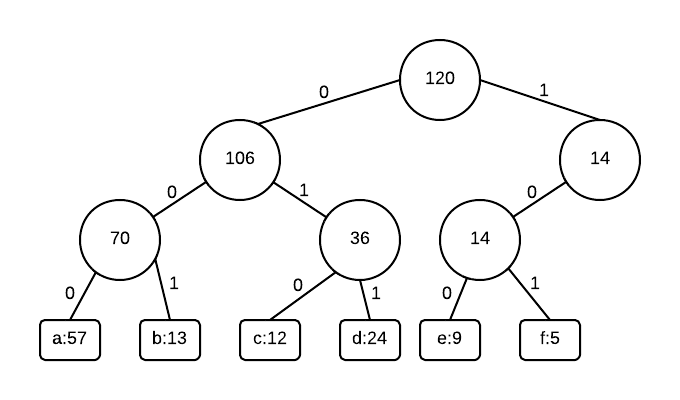
\includegraphics[width=100mm]{images/huff1.png}
\end{figure}

Tutti i caratteri sono foglie e sono allo stesso livello.
\linebreak
\linebreak
Esempio: codice a \textbf{lunghezza variabile}

\begin{center}
\begin{tabular}[htpd]{| l | c c c c c c |}

\hline
Carattere & a & b & c & d & e & f \\
Frequenza & 57 & 13 & 12 & 24 & 9 & 5 \\
Codice fisso & 0 & 101 & 100 & 111 & 1101 & 1100 \\
\hline
\end{tabular}
\end{center}

\begin{figure}[htpd]
\centering
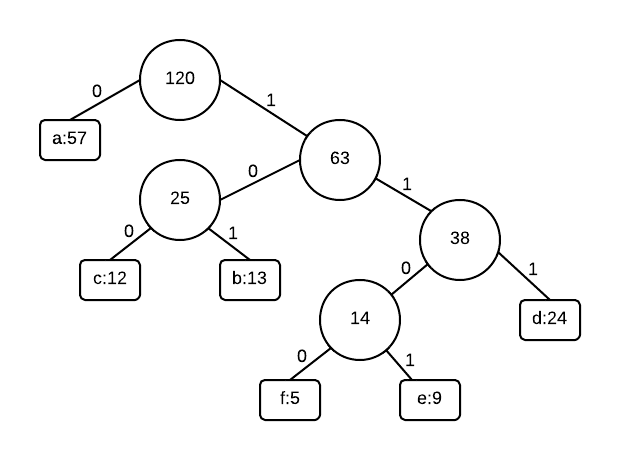
\includegraphics[width=100mm]{images/huff3.png}
\end{figure}

La lunghezza in bit del file codificato con il codice rappresentato da un albero $T$ è:

$$B(T)=\sum_{c\in\sum}f_cd_t(c)$$

dove $c\in\sum$ significa una sommatoria estesa a tutti i caratteri dell'alfabeto, $f_c$ è la frequenza del carattere $c$, $d_t(c)$ è la profondità della foglia che rappresenta il carattere $c$ nell'albero $T$.
\linebreak
\linebreak
\textbf{Nota}: assumiamo che l'alfabeto $\sum$ contenga almeno due caratteri. In caso contrario basata un numero per rappresentare il file: la sua lunghezza.

\subsection{Costruzione dell'albero del codice}

\begin{center}
\begin{tabular}[htpd]{| l | c c c c c c |}

\hline
Carattere & a & b & c & d & e & f \\
Frequenza & 57 & 13 & 12 & 24 & 9 & 5 \\
\hline
\end{tabular}
\end{center}

\begin{figure}[htpd]
\centering
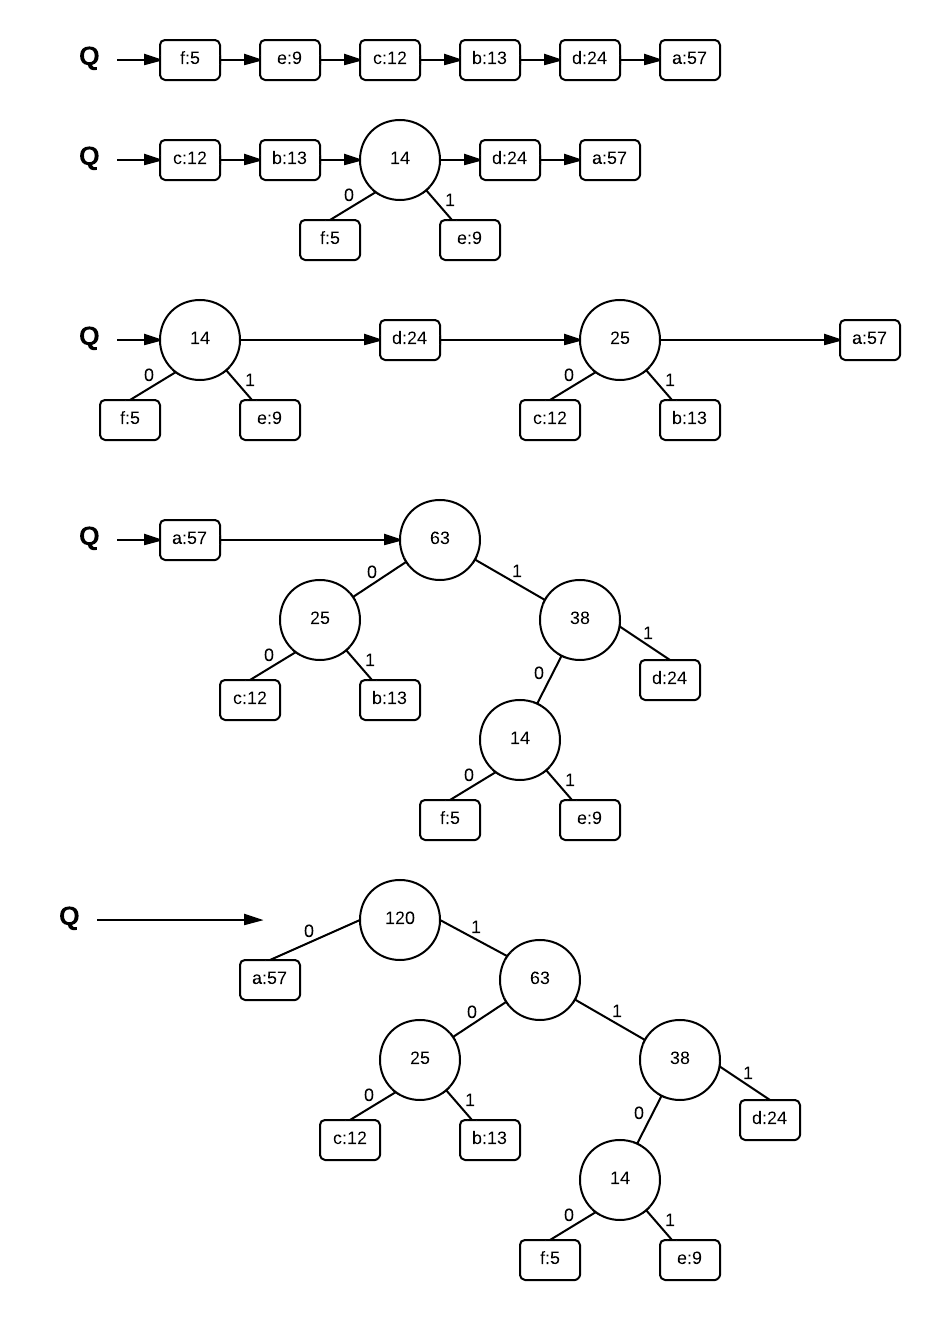
\includegraphics[width=100mm]{images/huff4.png}
\end{figure}

Vediamo di seguito l'algoritmo utilizzato per costruire l'albero:

\begin{lstlisting}[mathescape=true, caption=Huffman]

Huffman(c, f, n)
	Q = 0$\emptyset$
	for i=1 to n
		Push(Q, Nodo($f_i$, $c_i$))
	for j=n dowto 2
		x = ExtractMin(Q)
		y = ExtractMin(Q)
		Push(Q, Nodo(x,y))
	return ExtractMin(Q)

\end{lstlisting}

$Nodo(f,c)$ è il costruttore dei nodi foglia. $Nodo(x,y)$ è il costruttore dei nodi interni. La complessità dell'algoritmo è \textbf{$O(n\log n$}.
\linebreak
\linebreak
La tecnica di base per generare l'albero di un codice prefisso ottimo è quindi la seguente:

\begin{enumerate}

\item Ordinare la lista di caratteri per frequenza crescente;
\item Finchè la lista non contiene un solo elemento:
	\begin{enumerate}

	\item Estrarre i due caratteri con frequenza minore;
	\item Creare un nuovo albero che ha per figli i due caratteri del punto precedente e per radice la somma delle loro frequenze;
	\item Inserire l'albero nella lista (cancellando i fieli dalla lista).

	\end{enumerate}
\item Assegnare ad ogni carattere un codice secondo la definizione di albero del codice: un albero del codice è un albero binario le cui foglie sono i caratteri e una parola in codice viene interpretata come il cammino semplice dalla radice a quel carattere, dove 0 significa raggiungi il figlio sinistro e 1 significa raggiungi il figlio destro.
\end{enumerate}

\section{Analisi ammortizzata}

Si consideri il tempo richiesto per eseguire, nel \textbf{caso pessimo}, un'intera sequenza di operazioni. Se le operazioni costose sono relativamente meno frequenti allora il costo richiesto per eseguirle può essere ammortizzato con l'esecuzione delle operazioni meno costose.

\subsection{Metodo dell'aggregazione}

Si basa sul concetto di \textbf{costo ammortizzato}: data una sequenza di $n$ istruzioni aventi complessità $O(f(n))$, il costo ammortizzato della singola operazione si ottiene dividendo la complessità totale per il numero di istruzioni.

$$\hat{c}=\frac{O(f(n))}{n}$$

\subsection{Metodo degli accantonamenti (o dei crediti)}

Si caricano le operazioni meno costose di un costo aggiuntivo. Il costo aggiuntivo viene assegnato come \textbf{credito prepagato} a certi oggetti nella struttura dati. I crediti accumulati saranno usati per pagare le operazioni più costose su tali oggetti. 

Il costo ammortizzato delle operazioni meno costose è il costo effettivo aumentato del costo aggiuntivo. 

Il costo ammortizzato delle operazioni più costose è il costo effettivo diminuito del credito prepagato utilizzato.

Il costo artificiale fornisce un \textbf{limite superiore} al costo ammortizzato.

\subsection{Metodo del potenziale}

Si associa alla struttura dati $D$ un \textbf{potenziale} $\Phi(D)$ tale che la modifica della struttura dati dovuta alle operazioni meno costose comporti un aumento del potenziale, mentre le operazioni meno costose lo facciano diminuire.

Il costo ammortizzato è quindi la \textbf{somma algebrica} del costo effettivo e della variazione di potenziale. $D_i$ è la struttura dati dopo la \textit{c}-esima operazione e $c_i$ + il costo dell'\textit{i}-esima operazione.

$$\hat{c}_i=c_i+\Phi(D_i)-\Phi(D_{i-1})$$

Il costo ammortizzato di una sequenza di $n$ operazioni è:

$$\hat{c}=\sum_{i=1}^n\hat{c}_i=\sum_{i=1}^n[c_i+\Phi(D_i)-\Phi(D_{i-1})]$$
$$=c+\Phi(D_n)-\Phi(D_0)$$

Se la variazione $\Phi(D_n)-\Phi(D_0)$ del potenziale relativo all'esecuzione di tutta la sequenza non è negativa allora il costo ammortizzato $\hat{c}$ è una \textbf{maggiorazione} del costo reale $c$.

Altrimenti un valore $\Phi(D_n)-\Phi(D_0)$ negativo deve essere compensato con un aumento adeguato del costo ammortizzato delle operazioni.

\subsection{Esercizio 1}

Si vuole realizzare un contatore binario usando un array $A[0...k]$ per memorizzare i $k+1$ bit $b_k...b_1b_0$ della rappresentazione binaria del valore $x$ del contatore. Si vuole che il contatore possa iniziare anche con un valore maggiore di zero. A tale scopop si vuole che, oltre all'operazione \textbf{increment}, che aumenta di 1 il valore del contatore, sia prevista anche un'operazione iniziale \textbf{SET(A,n)}, che inizializza ad n il valore del contatore.
Usare il \textbf{metodo di aggregazione} per dimostrare che le operazioni di una sequenza costituita da una set seguita da $m$ increment, con $m=\Omega(k)$ hanno costo ammortizzato costante.
\linebreak
\linebreak
\textbf{Soluzione}:Vediamo anzitutto gli pseudo-codici delle due funzioni:

\begin{lstlisting}

Increment(A)
	i = 0
	while i<=k and A[i]==1
		A[i] = 0
		i++
	if i<=k
		A[i] = 1

\end{lstlisting}

\begin{lstlisting}

Set(A,n) // O(k)
	// PRE: A azzerato
	while i<=k and n>0
		A[i] = n%2
		n = n/2     // preso per difetto
		i++

\end{lstlisting}

Sia $\Phi(A)=$``numero di bit impostati a 1''. Il costo di una increment è $c=1+t$, dove $t\ge0$ è il numero di bit trasformati in 1 da 0. Sia $A_0$ lo stato iniziale del contatore azzerato ed $A_1$ il suo stato dopo aver eseguito una Set(A,n). Supponiamo di effettuare $m$ esecuzioni di increment per valutare l'analisi ammortizzata:

$$\Delta\Phi=\Phi(A_m)-\Phi(A_1)=t-1$$

Il numero di bit 1 rispetto ad $A_1$ varia di $-t+1$ in $A_m$. Dunque aggiungiamo $k$ alla formula per calcolare $\hat{c}$, distribuendolo a tutte le operazioni;

$$\hat{c}=c+\Phi(A_n)-\Phi(A_0)+\frac{k}{m}=1+t-t+1+\frac{k}{m}$$

Alla fine il costo ammortizzato è $O(1+\frac{k}{m})$, $m=\Omega(k), m\ge k$.

$$\frac{O(k)+O(1+\frac{k}{m})}{m+1}=O(\frac{k+1+k/m}{m+1})\le O(\frac{k+1+k/k}{k+1})=O(\frac{k+2}{k+1})=O(1)$$

\subsection{Esercizio 2}

Si vuole realizzare un timer usando un array $A$ per memorizzare i $k+1$ bit $b_k,....,b_1,b_0$ della rappresentazione binaria del valore del timer. Le operazioni previste per un timer sono \textit{Set(A,n)} che carica il timer ad $n$ secondi e \textit{Decrement(A)} che diminuisce di un secondo il valore del timer. L'operazione Set si può eseguire solamente quando il timer è azzerato mentre l'operazione Decrement si può eseguire soltanto quando il timer ha valore maggiore di 0. Scrivere le due funzioni Set e Decrement ed analizzarne la complessità ammortizzata.
\linebreak
\linebreak
\textbf{Suggerimento}: Memorizzare l'indice $m$ del bit 1 più significativo ($m=-1$ se tutti i bit sono 0, $m=k$ se tutti i bit sono a 1) ed usare come funzione potenziale il numero di bit uguali a 0 che precedono $A[m]$ più due volte il numero di bit che seguono $A[m]$ (che sono tutti 0), ossia $\Phi=\sum_{i=0}^{m-1}(1-b_i)+2(k-m)$.
\linebreak
\linebreak
\textbf{Soluzione}: Vediamo anzitutto gli pseudo-codici delle due operazioni:

\begin{lstlisting}

Set(A,n) // tutti i bit a 0, n<2^{k+1}
	k = A.lenght
	i = 0  // parto dal bit meno significativo
	while n>0 and i<=k
		A[i] = n%2  // il resto della divisione per 2
		n = n/2   // divisione intera per difetto
		i++
	if i>k
		error "underflow"
	else
		A.m = i-1

\end{lstlisting}

\begin{lstlisting}

Decrement(A)
	i = 0
	while A[i] == 0
		A[i] = 1
		i++
	A[i] = 0  // ora devo mettere apposto l'n
	if A.m == i
		A.m = A.m-1

\end{lstlisting}

\textbf{Analisi ammortizzata di Set}:

$$\hat{c}=c+\Delta\Phi$$
$$\Delta\Phi=\Phi+\Phi'=2(k-m)+\sum_{i=0}^{m-1}(1-b_i)-2(k+1)=$$
$$=2k-2m+\sum_{i=0}^{m-1}(1-b_i)-2k-2$$
$$\hat{c}\le m+1-2m+m-2 \le -1$$

Il costo è costante quindi ho concluso la dimostrazione.
\linebreak
\linebreak
\textbf{Analisi ammortizzata di Decrement}
\linebreak
\linebreak
$c=c+1$, proporzionale a $t-1$, dove $t$ è il numero di bit trasformati in 0.

$$\hat{c}=c+\Delta\Phi$$
$$\Delta\Phi=\Phi-\Phi'=2(k-m)+\sum_{i=0}^{m-1}(1-b_i)-2(k-m')+\sum_{i=0}^{m'-1}(1-b_i)=$$
$$-2m+2m'-t+1$$

$m$ ed $m'$ possono al massimo diversi tra loro di 1, quindi:

$$\Delta\Phi\le 2-t+1=3-t$$

$$\hat{c}=t+1+3-t=4$$

Ottengo un valore costante, inoltre:

$$\Phi_0=2(k+1)$$

In questo caso perchè il costo ammortizzato vada bene deve essere maggiore o uguale del costo reale.

Prendiamo le operazioni di segno:

$$\hat{c}_i=c_i+\Phi_i-\Phi_{i-1}$$
$$\sum_{i=1}^n\hat{c}_i=\sum_{i=1}^n\hat{c}_i+\Phi_n+\Phi_0\le\sum_{i=0}{n}(\hat{c}_i-\frac{\Phi_0}{n})$$
$$\hat{c}_i=c_i+\frac{\Phi_0}{n}$$

Devo distribuire, il costo ammortizzato è quindi:

$$\hat{c}=4+\frac{2(k+1)}{n}$$
Se $n=\Omega(k) \Rightarrow \hat{c}=O(1)$

\section{B-alberi}

I B-alberi sono \textbf{alberi bilanciati} adatti per memorizzare grandi masse di dati in memoria secondaria. Sono simili agli alberi rosso-neri, ma sono progettati per minimizzare gli accessi alla memoria secondaria. Le operazioni sono \textbf{insert}, \textbf{delete}, \textbf{search}, \textbf{split} e \textbf{join}.

I nodi dei B-alberi possono avere un numero di chiavi $n\ge 1$ ed $n+1$ figli.

\begin{figure}[htpd]
\centering
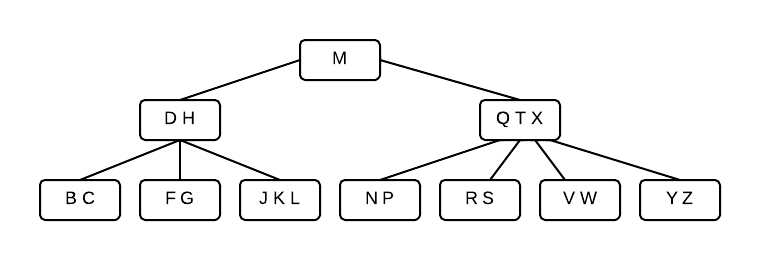
\includegraphics[width=100mm]{images/b-alberi1.png}
\end{figure}

\subsection{Definizione di un B-albero}

Un B-albero $T$ è un albero di radice $T.root$ tale che:

\begin{enumerate}

\item Ogni nodo $x$ contiene i seguenti campi:
	\begin{enumerate}
	\item $x.n$: il numero di chiavi presenti nel nodo;
	\item $x.key_1\le x.key_2 \le ... \le x.key_n $: le $x.n$ chiavi in ordine crescente;
	\item $x.leaf$: valore booleano che è true se il nodo $x$ è una foglia, false altrimenti.
	\end{enumerate}
\item Se il nodo non è una foglia contiene anche $x.c_1, X.c_2, x.c_{n+1}$: gli $n+1$ puntatori ai figli;
\item Le chiavi $x.key_1, x.key_2, ..., x.key_n$ di un nodo interno separano le chiavi dei sottoalberi. Se $k_i$ è una chiave qualsiasi del sottoalbero $x.c_i$, allora:

$$k_1 \le x.key_1 \le k_2 \le x.key_2 \le ... \le x.key_{x.n} \le k_{x.n+1}$$

\item Le foglie sono tutte alla stessa profondità $h$, detta \textbf{altezza dell'albero};
\item Vi sono limiti inferiori e superiori al numero di chiavi in un nodo, e tali limiti dipendono da una costante $t$ detta \textbf{grado minimo} del B-albero.
	\begin{enumerate}
	\item Ogni nodo, eccetto la radice, ha almeno $t-1$ chiavi e, se non è una foglia, ha almeno $t$ figli;
	\item Se l'albero non è vuoto la radice contiene almeno una chiave;
	\item Ogni nodo ha al più $2t-1$ chiavi e, se non è foglia, ha al più $2t$ figli.
	\end{enumerate}

\end{enumerate}

Ad ogni chiave sono generalmente associate delle informazioni ausiliarie. Assumeremo implicitamente che quando viene copiata una chiave vengono copiate anche tali informazioni. I B-alberi più semplici sono quelli con grado minimo $t=2$. Ogni nodo interno ha 2,3 o 4 figli.
Ogni albero non vuoto di grado minimo $t$ con $N$ chiavi ha altezza:

$$h \le \log_t\frac{N+1}{2}$$

\subsection{Operazioni sui B-alberi}

Adottiamo le seguenti convenzioni per le operazioni sui B-alberi:

\begin{enumerate}

\item La radice del B-albero è sempre in memoria;
\item I nodi passati come parametri alle procedure sono stati preventivamente caricati in memoria.

\end{enumerate}

\subsubsection{Creazione di un B-albero vuoto}

La procedura ausiliaria \textbf{ALLOCATE-NODE} alloca una pagina del disco da utilizzare come nuovo nodo nel tempo $O(1)$. Supponiamo che un nodo creato da ALLOCATE-NODE non richieda l'operazione DISK-WRITE.

\begin{lstlisting}[caption=Creazione di un B-albero]

B-TREE-CREATE(T)
	x = ALLOCATE-NODE()
	x.leaf = true
	x.n = 0
	DISK-WRITE(x)
	T.root = x

\end{lstlisting}

La procedura B-TREE-CREATE richiede $O(1)$ operazioni su disco e quindi un tempo di CPU pari a $O(1)$.

\subsubsection{Ricerca in un B-albero}

\begin{lstlisting}[mathescape=true, caption=Ricerca in un B-albero]

B-TREE-SEARCH(x, k)
	i = 1
	while i $\le$ x.n and k > $x.key_i$
		i = i+1
	if i$\le$ x.n and k == $x.key_i$
		return(x, i)
	elseif x.leaf
		return nil
	else DISK-READ(x,$c_i$)
		return B-TREE-SEARCH($x.c_i$, k)

\end{lstlisting}

La procedura richiede tempo $O(\log_2 N)$. Il numero di $DISK-READ$ è al più uguale all'altezza $h$ dell'albero, quindi $O(\log_tN)$. Il tempo di CPU della procedura è:

$$T\le(h+1)\log_2(2t-1)$$
$$=O(\log_tN\log_2t)$$
$$=O(\log_2N)$$

\subsubsection{Inserimento di una chiave}

L'aggiunta di  una chiave ad un B-albero può avvenire soltanto in una foglia e soltanto se la foglia non è piena, cioè non ha il numero massimo $2t-1$ di chiavi. Possiamo garantirci che la foglia a cui arriveremo non sia piena se ad ogni passo nella discesa dalla radice ci assicuriamo che il figlio su cui scendiamo non sia pieno. Nel caso in cui tale figlio sia pieno chiamiamo prima una particolare funzione \textbf{$SPLIT-CHILD$} che lo divide in due.

\begin{lstlisting}[mathescape=true, caption=Procedura di divisione di un nodo]

B-TREE-SPLIT-CHILD(x, i)
	z = ALLOCATE-NODE()
	y = $x.c_i$
	z.leaf = y.leaf
	z.n = t-1
	for j=1 to t-1
		$z.key_j$ = $y.key_{j+t}$
	if not y.leaf
		for j=1 to t
			$z.c_j$ = $y.c_{j+t}$
	y.n = t-1
	for j=x.n+1 downto i+1
		$x.c_{j+1}$ = $x.c_j$
	$x.c_{i+1}=z$
	for j=x.n downto i
		$x.key_{j+1}=x.key_j$
	$x.key_i=y.key_t$
	x.n = x.n+1
	DISK-WRITE(y)
	DISK-WRITE(z)
	DISK-WRITE(x)

\end{lstlisting}

Inseriamo ora una chiave $k$ nel B-albero $T$ di altezza $h$ con un singolo passaggio in discesa nell'albero, richiedendo $O(h)$ accessi. Il tempo di CPU richiesto è $O(th)=O(t\log_tn)$. La procedura B-TRSERT usa B-TREE-SPLIT-CHILD per garantire che la ricorsione non arrivi mai a un nodo pieno.

\begin{lstlisting}[mathescape=true, caption=Inserimento di una chiave]

B-TREE-INSERT(T,k)
	r = T.root
	if r.n == 2t-1
		s = ALLOCATE-NODE()
		T.root = s
		s.leaf = false
		s.n = =
		s.$c_1$ = r
		B-TREE-SPLIT-CHILD(s,1)
		B-TREE-INSERT-NONFULL(s,k)
	else
		B-TREE-INSERT-NONFULL(r,k)

\end{lstlisting}

La procedura finisce chiamando B-TREE-INSERT-NONFULL per inserire la chiave $k$ nell'albero che ha un nodo radice non pieno. La procedura B-TREE-INSERT-NONFULL effettua la ricorsione quante volte serve per discendere l'albero, assicurandosi che il nodo in cui effettua la ricorsione non sia mai pieno, chiamando B-TREE-SPLIT-CHILD se necessario.

\begin{lstlisting}[mathescape=true, caption=B-Tree insert nonfull]

B-TREE-INSERT-NONFULL(x,k)
	i = x.n
	if x.leaf
		while $i\ge 1$ and k<$x.key_i$
			x.$key_{i+1}$ = x.$key_i$
			i = i-1
		x.$key_{i+1}$=k
		x.n = x.n+1
		DISK-WRITE(x)
	else while $i\ge 1$ and k<x.$key_i$
			i = i-1
		i = i+1
		DISK-READ(x.$c_i$)
		if $x.c_i$.n == 2t-1
			B-TREE-SPLIT-CHILD(x,i)
			if k>$x.key_i$
				i = i+1
			B-TREE-INSERT-NONFULL(x.$c_i$,k)

\end{lstlisting}

Il tempo totale della CPU è $O(th)=O(t\log_tn)$.

\subsubsection{Cancellazione di una chiave}

La cancellazione di una chiave da un B-albero è analoga all'inserimento, ma un po' più complicata, perchè una chiave può essere cancellata da un nodo qualsiasi e l'eliminazione di una chiave da un nodo interno richiede che i figli del nodo vengano riorganizzati. Azichè lo pseudocodice, descriveremo il funzionamento dell'operazione di cancellazione.

\begin{enumerate}

\item Se la chiave si trova nel nodo $x$ e $x$ è una foglia, cancellare la chiave $k$ da $x$;
\item Se la chiave $k$ si trova nel nodo $x$ e $x$ è un nodo interno, eseguire le seguenti operazioni:
	\begin{enumerate}
	\item Se il figlio $y$ che precede $k$ nel nodo $x$ ha almeno $t$ chiavi, trovare il predecessore $k'$ di $k$ nel sottoalbero con radice in $y$. Cancellare ricorsivamente $k'$ e sostituire $k$ con $k'$ in $x$;
	\item Simmetricamente, se il figlio $z$ che segue $k$ nel nodo $x$ ha almeno $t$ chiavi, trovare il successore $k'$ di $k$ nel sottoalbero con radice in $z$. Cancellare ricorsivamente $k'$ e sostituire $k$ con $k'$ in $x$;
	\item Altrimenti, se entrambi i nodi $y$ e $z$ hanno soltanto $t-1$ chiavi, fondere $k$ e tutto $z$ nel nodo $y$, in modo che $x$ perda sia $k$ sia il puntatore a $z$; adesso $y$ contiene $2t-1$ chiavi. Poi, rilasciare $z$ e cancellare ricorsivamente $k$ da $y$.
	\end{enumerate}
\item Se la chiave $k$  non è presente nel nodo interno $x$, determinare la radice $x.c_i$ del sottoalbero appropriato che deve contenere $k$, se $k$ è davvero presente nell'albero. Se $x.c_i$ ha soltanto $t-1$ chiavi, eseguire il passo 3a o 3b, se necessario, per avere la garanzia di arrivare a un nodo che contiene almeno $t$ chiavi. Poi, finire effettuando la ricorsione sul figlio appropriato di $x$.
	\begin{enumerate}
	\item Se $x.c_i$ ha soltanto $t-1$ chiavi, ma ha un fratello adiacente con almeno $t$ chiavi, assegnare a $x.c_i$ una chiave extra, spostando in basso una chiave da $x$ in $x.c_i$, spostando in alto una chiave dal fratello sinistro o destro di $x.c_i$ in $x$ e, infine, spostando in $x.c_i$ un puntatore al figlio del fratello (quello adiacente alla chiave spostata);
	\item Se $x.c_i$ ed entrambi i fratelli adiacenti di $x.c_i$ hanno $t-1$ chiavi, fondere $x.c_i$ con un fratello in un nuovo nodo; questo richiede che una chiave venga spostata in basso da $x$ nel nuovo nodo per diventare la chiave mediana di questo nodo.
	\end{enumerate}
\end{enumerate}

\subsection{Esercizi}

\subsubsection{Esercizio 1}

Mostrare come sia possibile aggiungere ad ogni nodo interno $x$ di un B-albero i campi $x.size_i$ che contengono il numero di chiavi presenti nei sottoalberi di radici $x.c_i$. Dire quali sono le modifiche da apportare a Insert e Delete. Assicurarsi che la complessità asintotica non aumenti.
\linebreak
\linebreak
\textbf{Soluzione}: Sia $x$ un nodo interno e sia $y=x.c_i$ figlio di $x$. Vale la seguente formula:

$$
x.size_i=
\begin{cases}
y.n, & y foglia \\
y.n+\sum_{j=1}^{y.n+1}y.size_j & altrimenti
\end{cases}
$$

Insert percorre un cammino dalla radice fino alla foglia in cui si deve inserire la nuova chiave. Prima di scendere da un nodo $x$ al figlio $x.c_i$ aumentiamo $x.size_i$ di 1.

Quando eseguiamo una SplitChil(x,i,$x.c_i$) dobbiamo ricalcolare sia $x.size_i$ che $x.size_{i+1}$ usando la formula precedente.

Delete percorre un cammino dalla radice fino alla foglia da cui viene rimossa o la chiave data o la successiva. Prima di scendere da un nodo $x$ al figlio $x.c_i$ diminuiamo $x.size_i$ di 1.

Quando eseguiamo una AugmentChild dobbiamo usare la formula precedente per ricalcolare i campi $x.size_i$ relativi ai figli che vengono modificati.

\subsubsection{Esercizio 2}

Aumentare la struttura dati B-albero aggiungendo ad ogni nodo $x$ i campi $x.sumkey_i=1,...,x.n+1$ che contengono la somma delle chiavi presenti nel sottoalbero di radice $x.c_i$. Dire quali modifiche occorre apportare alle operazioni Insert e Delete per mantenere aggiornati tali campi senza aumentare la complessità asintotica di tali operazioni.
\linebreak
\linebreak
\textbf{Soluzione}: sia $x$ un nodo interno e sia $y=x.c_i$ figlio di $x$. Vale la seguente formula:

$$x.sumkey_i=
\begin{cases}
\sum_{j=1}^{y.n}y.key_j & y foglia \\
\sum_{j=1}^{y.n}y.key_j+\sum_{j=1}^{y.n+1}y.sumkey_j & altrimenti
\end{cases}
$$

Insert percorre un cammino dalla radice fino alla foglia in cui si deve inserire la nuova chiave. Prima di scendere da un nodo $x$ al figlio $x.c_i$, aumentiamo $x-.sumkey_i$ del valore della chiave che si vuole inserire.

Quando eseguiamo una SplitChild(x,i,$x.c_i$) dobbiamo ricalcolare sia $x.sumkey_i$ che $x.sumkey_{i+1}$ usando la formula precedente.

Delete percorre un cammino dalla radice fino alla foglia da cui viene rimossa o la chiave data o la successiva. Prima di scendere da un nodo $x$ al figlio $x.c_i$ diminuiamo $x.sumkey_i$ del valore della chiave da cancellare.

Quando eseguiamo una AugmentChild(x,i,$x.c_i$) dobbiamo usare la formula precedente per ricalcolare i campi $x.sumkey_i$ relativi ai figli che vengono modificati.

\subsubsection{Esercizio 3}

Aumentare la struttura dati B-albero aggiungendo ad ogni nodo $x$ i campi $x.maxkey_i$, $i=1,...,x.n+1$ che contengono la massima chiave presente nel sottoalbero di radice $x.c_i$. Dire quali modifiche occorre apportare alle operazioni Insert e Delete per mantenere aggiornati tali campi senza aumentare la complessità asintotica di tali operazioni.
\linebreak
\linebreak
\textbf{Soluzione}: Sia $x$ un nodo interno e sia $y=x.c_i$ figlio di $x$. Vale la seguente formula:

$$
x.maxkey_i=
\begin{cases}

max_{1\le i \le y.n}(y.key_i) & y foglia \\
max(max_{1\le j \le y.n}(y.key_j)) \\
max_{1\le h \le y.n+1}(y.maxkey_h) & altrimenti

\end{cases}
$$

Insert percorre un cammino dalla radice fino alla foglia in cui si deve inserire la nuova chiave. Prima di scendere da un nodo $x$ al figlio $x.c_i$, confrontiamo $x.maxkey_i$ con il valore della chiave che si vuole inserire.

Quando eseguiamo una SplitChild(x,i,$x.c_i$) dobbiamo ricalcolare sia $x.maxkey_i$ che $x.maxkey_{i+1}$ usando la formula precedente.

Delete percorre un cammino dalla radice fino alla foglia da cui viene rimossa o la chiave data o la successiva. Al ritorno dalla chiamata ricorsiva da nodo $x$ al figlio $x.c_i$ ricalcoliamo $x.maxkey_i$ se si deve cancellare proprio $x.maxkey_i$.

Quando eseguiamo una AugmentChild(x,i,x,$c_i$) dobbiamo usare la formula precedente per ricalcolare i campi $x.maxkey_i$ relativi ai figli che vengono modificati.

\subsubsection{Esercizio 4}

Scrivere una funzione Search che dato un B-albero $T$ ed un valore $v$ cerca la minima chiave $k>v$. La funzione deve ritornare il puntatore al nodo che contiene la chiave $k$ e la posizione di tale chiave nel nodo. Deve ritornare $nil$ se $T$ non contiene alcuna chiave maggiore di $v$.
\linebreak
\linebreak
\textbf{Soluzione}:

\begin{lstlisting}[mathescape=true]

Search(x,v)
	i = 1
	while i $\le$ n and $x.key_i \le v$
		i = i+1
	if i == x.n+1
		if $x.c_i$ == nil
			return nil
		else
			DiskRead($x.c_i$)
			return Search($x.c_i$,v)
	else // $x.key_i$ > v
		if $x.c_i$ == nil
			return (x, i)
		else
			DiskRead($x.c_i$)
			(y, j) = Search($x.c_i$, v)
			if y == nil
				return (x, i)
			else
				return (y, j)

\end{lstlisting}

%\appendix

%\input{glossario}


\end{document}